\documentclass[../momento_1.tex]{subfiles}

Esta fase tem como objetivo a implementação da operação de \textit{reset} da matriz $M_{t,k}$ e, por consequência da tabela de números aleatórios.   operação  de 
\textit{reset} consiste  em  reiniciar  a  matriz $M_{t,k}$ com  as sementes  do  ficheiro indicado  no ficheiro  de  configuração. Esta operação só pode ser executada no agente quando é feita uma operação de \textit{snmpset}
 à correspondente instância do objeto escalar do tipo string do grupo \textit{unpredictableParam} e só é autorizada se o valor da \textit{string} no pedido \textit{snmpset} for igual chave de configuração. Após a execução da operação \textit{reset}, o agente pausa as suas operações de refrescamento por $R*10$ segundos e retoma a operação de refrescamento a cada $1/T$ segundos.\par
 
Para implementar a operação de \textit{reset} a chave de configuração usada no arranque do agente é guardada na variável \textit{cc} que é usada para comparar com a \textit{string} colocada na instância \textit{unpredicatableReset} quando executado um comando \textit{snmpset} pelo utilizador. Se for igual pausa as operações de refrescamento senão continua, como exemplificado no Exemplo \ref{lst:reset}.\\

{\setstretch{1.1}
\begin{lstlisting}[caption={Exemplo Comparação da chave de configuração e pausa das operações de refrescamento},label={lst:reset},language=JAVA]
	 
        MOChangeListener l = new MOChangeListener() {
            public void beforePrepareMOChange(MOChangeEvent moChangeEvent) {}
            public void afterPrepareMOChange(MOChangeEvent moChangeEvent) {}
            public void beforeMOChange(MOChangeEvent moChangeEvent) {}
            public void afterMOChange(MOChangeEvent moChangeEvent) {
                if (uminhogrmib.getUnpredictableReset().getValue().equals(getOctetString(cc))) {
                    uminhogrmib.getUnpredictableReset().setValue(getOctetString(""));
                    u = 0;
                    timers.cancelTimer();
                    try {
                        reset();
                    } catch (IOException e) {
                        e.printStackTrace();
                    }
                    try {
                        timers.startTimer(delay, interval);
                    } catch (IOException e) {
                        e.printStackTrace();
                    }
                }
            }
        };
\end{lstlisting}}


Para detetar um \textit{set} à instância \textit{unpredictableReset} foi implementado um \textit{listener} descrito no exemplo \ref{lst:reset} que é executado assim que esta instância for alterada. No caso de pausar as operações de refrescamento, implementou-se um \textit{Timer} que só é executada após \textit{delay} segundos e re-executada em \textit{interval} segundos. A classe \textit{RefreshTimer} encontra-se exemplificada no exemplo \ref{lst:timer}.\\

{\setstretch{1.1}
\begin{lstlisting}[caption={Exemplo Classe \textit{RefreshTimer}},label={lst:timer},language=JAVA]
	 
        public class RefreshTimer {
    private Timer timer;
    
    public void startTimer(int delay, long interval) throws IOException{
        this.timer= new Timer();
        SNMPAgent agent = new SNMPAgent("0.0.0.0/6666");
        
        timer.schedule(new TimerTask() {
            @Override
            public void run() {
                agent.refresh();
            }
        }, delay,interval);
    }
    
    public void cancelTimer(){
        this.timer.cancel();
    }
}
\end{lstlisting}}

Para demonstrar o seu funcionamento, na função \textit{refresh} uma variável está sempre a incrementar sempre que o método \textit{refresh()} é executado e quando é realizada uma operação de \textit{reset} a matriz $M_{t,k}$ é reiniciada, como podemos observar na Figura \ref{fig:setTimer}.\\

\begin{figure}[H]
\centering
\captionsetup{justification=centering,margin=4cm}
\centerline{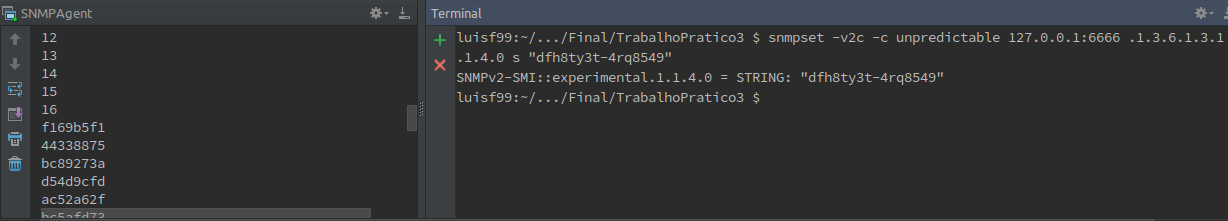
\includegraphics[scale=0.4]{../imagens/setTimer.png}}
\caption{Grupo \textit{unpredictableTable}.}
\label{fig:setTimer}
\end{figure}